\subsection{Changes in numerical solutions in time}
	This section discuss how numerical solutions accuracy changes in time. For each of the schemes grid size is equal to $400$ in order to decrease quantization errors.
\begin{figure}[!htbp]
	\begin{subfigure}[b]{0.5\textwidth}
		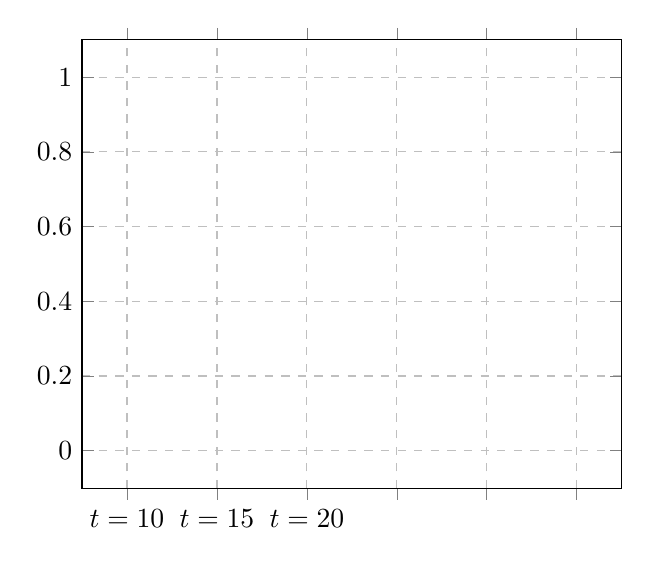
\begin{tikzpicture}
			\begin{axis}[
				ybar,
				%symbolic x coords={5,10,15,20},
				xticklabels={$t=5$,$t=10$,$t=15$,$t=20$},
				xtick=data,
			%	enlarge x limits={abs=2cm},
				ymajorgrids=true,
				xmajorgrids=true,
				grid style=dashed,
				legend pos=north west
				%legend style={at={(0.5,-0.1)},anchor=north,legend cell align=left},
				%nodes near coords,
				%every node near coord/.append style={rotate=90, anchor=west},
				]
				\addcustomybarplot{../Code/results/changeInTime/explicit-upwind-400-exp.conf-norms.csv}{2}{red}{Exponent};
				\addcustomybarplot{../Code/results/changeInTime/explicit-upwind-400-sign.conf-norms.csv}{2}{green}{Signum};						
			\end{axis}
		\end{tikzpicture}
		\caption{Explicit upwind scheme, $CFL=0.98$}
	\end{subfigure}
	\begin{subfigure}[b]{0.5\textwidth}
		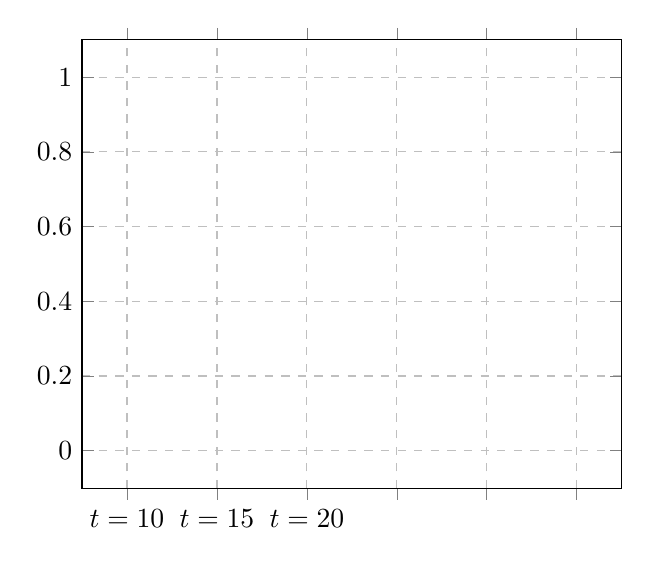
\begin{tikzpicture}
			\begin{axis}[
				ybar,
				%symbolic x coords={5,10,15,20},
				xticklabels={$t=5$,$t=10$,$t=15$,$t=20$},
				xtick=data,
			%	enlarge x limits={abs=2cm},
				ymajorgrids=true,
				xmajorgrids=true,
				grid style=dashed,
				legend pos=north west
				%legend style={at={(0.5,-0.1)},anchor=north,legend cell align=left},
				%nodes near coords,
				%every node near coord/.append style={rotate=90, anchor=west},
				]
				\addcustomybarplot{../Code/results/changeInTime/implicit-upwind-400-exp.conf-norms.csv}{2}{blue}{Exponent};
				\addcustomybarplot{../Code/results/changeInTime/implicit-upwind-400-sign.conf-norms.csv}{2}{black}{Signum};						
			\end{axis}
		\end{tikzpicture}
		\caption{Implicit upwind scheme, $CFL=0.07$}
	\end{subfigure}
	\begin{subfigure}[b]{0.5\textwidth}
		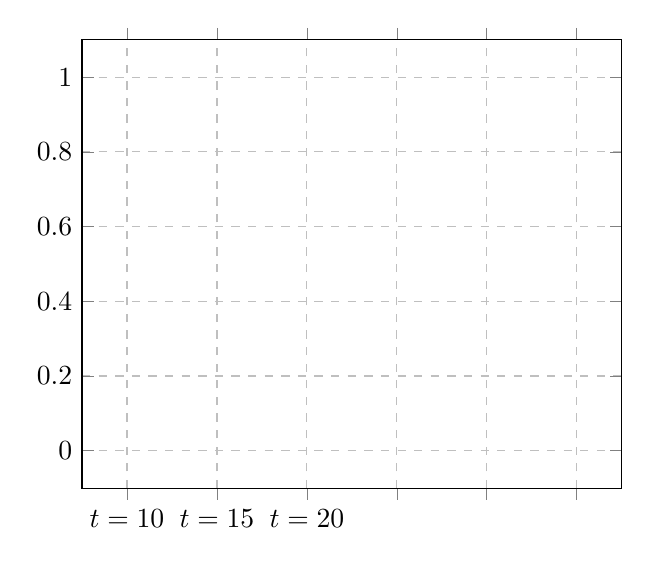
\begin{tikzpicture}
			\begin{axis}[
				ybar,
				%symbolic x coords={5,10,15,20},
				xticklabels={$t=5$,$t=10$,$t=15$,$t=20$},
				xtick=data,
			%	enlarge x limits={abs=2cm},
				ymajorgrids=true,
				xmajorgrids=true,
				grid style=dashed,
				legend pos=north west
				%legend style={at={(0.5,-0.1)},anchor=north,legend cell align=left},
				%nodes near coords,
				%every node near coord/.append style={rotate=90, anchor=west},
				]
				\addcustomybarplot{../Code/results/changeInTime/lax-wendroff-400-exp.conf-norms.csv}{2}{yellow}{Exponent};
				\addcustomybarplot{../Code/results/changeInTime/lax-wendroff-400-sign.conf-norms.csv}{2}{brown}{Signum};						
			\end{axis}
		\end{tikzpicture}
		\caption{Lax-Wendroff scheme, $CFL=0.98$}
	\end{subfigure}
	\begin{subfigure}[b]{0.5\textwidth}
		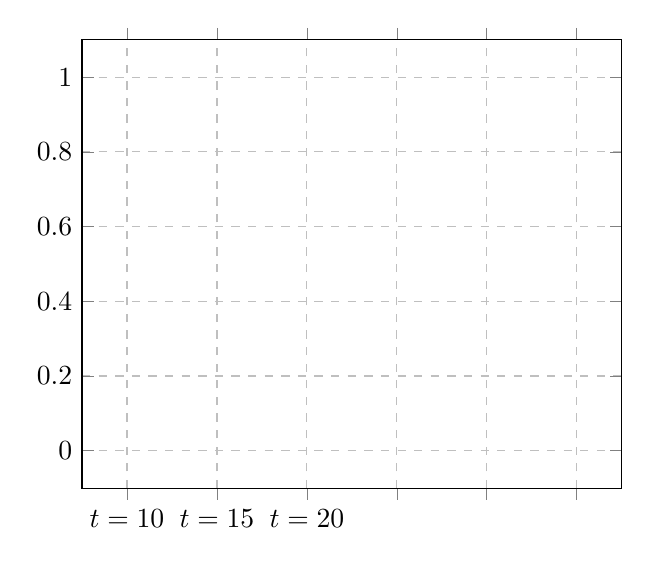
\begin{tikzpicture}
			\begin{axis}[
				ybar,
				%symbolic x coords={5,10,15,20},
				xticklabels={$t=5$,$t=10$,$t=15$,$t=20$},
				xtick=data,
			%	enlarge x limits={abs=2cm},
				ymajorgrids=true,
				xmajorgrids=true,
				grid style=dashed,
				legend pos=north west
				%legend style={at={(0.5,-0.1)},anchor=north,legend cell align=left},
				%nodes near coords,
				%every node near coord/.append style={rotate=90, anchor=west},
				]
				\addcustomybarplot{../Code/results/changeInTime/richtmyer-ms-400-exp.conf-norms.csv}{2}{purple}{Exponent};
				\addcustomybarplot{../Code/results/changeInTime/richtmyer-ms-400-sign.conf-norms.csv}{2}{orange}{Signum};
										
			\end{axis}
		\end{tikzpicture}
		\caption{Richtmyer multi-step scheme, $CFL=1.96$}
	\end{subfigure}
	\caption{Comparison of distribution of error (norm 1) for different schemes among different time steps, for given CFL numbers.}
	\label{fig:normsInTime}
\end{figure}